\documentclass[11pt]{article}
\usepackage[shortlabels]{enumitem}
\usepackage[margin=1in,headheight=15pt]{geometry}   % Adjusted headheight
\usepackage{amsmath}
\usepackage{fancyhdr}
\usepackage{graphicx}
\usepackage{cancel}
\usepackage{amsfonts}
\usepackage{setspace}

% Set up fancy header/footer
\pagestyle{fancy}
\fancyhead[LO,L]{Jimmy Chen}
\fancyhead[CO,C]{CSCI 2500 - Computer Organization}
\fancyhead[RO,R]{November 30, 2023}
\fancyfoot[LO,L]{}
\fancyfoot[CO,C]{\thepage}
\fancyfoot[RO,R]{}
\renewcommand{\headrulewidth}{0.4pt}
\renewcommand{\footrulewidth}{0.4pt}
\graphicspath{ {./images/} }
\onehalfspacing

\begin{document}
\section{Homework 4}


\setcounter{section}{12}
\setcounter{subsection}{13}
\subsection{Excersises}

\setcounter{subsubsection}{4}
\subsubsection{Question 5}
In the exercise, we examine in detail how an instruction is executed in single-cycle datapath. Problems in this exercise refer to a clock cycle in which the processor fetches the following instruction word: 0xadac0014.\\
For context: The encoded instruction is \textbf{sw \$t4, 20(\$t5)}

\begin{enumerate}[(a)]
    \item What are the values of the ALU control unit's inputs for this instruction?\\
    \textbf{Work:}
    \begin{center}
        Opcode: 0xadac // Opcode for sw\\
        Source Register (\$t5)L 0x00\\
        Destination Register (\$t4): 0x10\\
        Offset: 20\\
        ALUOperation: 10 (Add)\\
        ALUSrc (ALU source): 1 (Immediate value from instruction)\\
        Function: 0 (Not used)\\
        \fbox{\begin{minipage}{24em}
            \begin{center}
                \Large{\textbf{Answer: ALU Control Input: 101}}
            \end{center}
        \end{minipage}}
    \end{center}

    \item What is the new PC address after this instruction is executed? Highlight the path through which this value is determined.\\
    \textbf{Work:}
    \begin{center}
        ALU operand 1: PC value\\
        ALU operand 2: 4 // Constant value to add \\
        \fbox{\begin{minipage}{35em}
            \begin{center}
                \Large{\textbf{Answer: The new will be the old PC address + 4.}}
            \end{center}
        \end{minipage}}
    \end{center}

    \item For each mux, show the values of its inputs and outputs during the execution of this instruction. List values that are register outputs at \textbf{Reg [xn]}\\
    \textbf{Answer:}\\[0.15in]
    Mux1 (ALU Source):
    \begin{itemize}
        \item Input 0: PC + 4
        \item Input 1: Sign-extended offset
        \item Output: Sign-extended offset
    \end{itemize}
    Mux2 (Write Register):
    \begin{itemize}
        \item Input 0: Register \$t4's number // dest reg
        \item Input 1: Register \$t5's number // src reg
        \item Selected Input: 0 // since we're writing to \$t4
    \end{itemize}
    Mux3 (Write Data):
    \begin{itemize}
        \item Input 0: ALU result // memory address to store data
        \item Input 1: Register \$t4's value // data to be stored in memory
        \item Selected Input: 1 // since we're writing to \$t4
    \end{itemize}

    \item What are the input values for the ALU and the two add units?\\
    \textbf{Answer:}
    \begin{center}
        ALU input 1: Value from register \$t5 //from Mux 1, input 1\\
        ALU input 2: Offset of 20 //immediate value from instruction\\
        Add Unit input 1: Value from register \$t5 //from Mux 1, input 1\\
        Add Unit input 2: Offset of 20 //immediate value from instruction\\
    \end{center}
    \item What are the values of all inputs for the registers unit?\\
    \textbf{Answer:}
    \begin{center}
        Read Register 1: Value from register \$t4 (from Mux2, input 0) 0x10\\
        Read Register 2: Value from register \$t5 (from Mux1, input 1) 0x00\\
        Write Register: Value from register \$t4 (from Mux2, input 0) 0x10\\
        Write Data: Value from register \$t4 (from Mux3, input 1)\\
        RegWrite: 1 or Active // since we're writing to \$t4\\
    \end{center}
\end{enumerate}


\setcounter{subsubsection}{6}
\subsubsection{Question 7}
Problems in this exercise assume that the logic blocks used to implement a processor's datapath (COD Figure 4.21) have the following latencies:
\begin{center}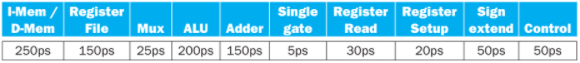
\includegraphics[scale=0.6]{q7_image}\\\end{center}
"Register read" is the time needed after the rising clock edge for the new register value to appear on the output. This value applies to the PC only. "Register setup" is the amount of time a register's data input must be stable before the rising edge of the clock. This value applies to both the PC and Register File.

\begin{enumerate}[(a)]
    \item What is the latency of an R-type instruction(i.e., how long must the clock period be to ensure that this instruction works correctly)?\\
    \textbf{Answer:}
    \begin{center}
        R-type Instruction Equation: Reg. File + I-Mem/D-Mem + (Mux * 2) + ALU + Reg. Read + Reg. Setup\\
        150ps + 250ps + 50ps + 200ps + 30ps + 20ps = 700ps\\
        \fbox{\begin{minipage}{15em}
            \begin{center}
                \Large{\textbf{Answer: 700ps}}
            \end{center}
        \end{minipage}}
    \end{center}
    
    \item What is the latency of lw? (Check your answer carefully. Many students place extra muxes on the critical path.)\\
    \textbf{Answer:}
    \begin{center}
        Latency of lw Equation = Reg. Read + (I-Mem/D-Mem * 2) + Reg. File + ALU + (2 * Mux) + Reg. Setup\\
        30ps + 500ps + 150ps + 200ps + 50ps + 20ps = 950ps\\
        \fbox{\begin{minipage}{15em}
            \begin{center}
                \Large{\textbf{Answer: 950ps}}
            \end{center}
        \end{minipage}}
    \end{center}

    \item What is the latency of sw? (Check your answer carefully. Many students place extra muxes on the critical path.)\\
    \textbf{Answer:}
    \begin{center}
        Latency of sw Equation = Reg. Read + (I-Mem/D-Mem * 2) + Reg. File + ALU + Mux\\
        30ps + 500ps + 150ps + 200ps + 25ps = 905ps\\
        \fbox{\begin{minipage}{15em}
            \begin{center}
                \Large{\textbf{Answer: 905ps}}
            \end{center}
        \end{minipage}}
    \end{center}

    \item What is the latency of beq?\\
    \textbf{Answer:}
    \begin{center}
        Latency of beq Equation = Reg. Read + I-Mem/D-Mem + Reg. File + ALU + (Mux * 2) + Single Gate + Reg. Setup\\
        30ps + 250ps + 150ps + 50 + 200ps + 5ps + 20ps = 705ps\\
        \fbox{\begin{minipage}{15em}
            \begin{center}
                \Large{\textbf{Answer: 705ps}}
            \end{center}
        \end{minipage}}
    \end{center}

    \item What is the latency of an arithmetic, logical, or shift I-type (non-load) instruction?\\
    \textbf{Answer:}
    \begin{center}
        Latency of I-type Equation = Reg. Read + I-Mem/D-Mem + Reg. File + ALU + (Mux * 2) + Reg. Setup\\
        30ps + 250ps + 150ps + 200ps + 50ps + 20ps = 700ps\\
        \fbox{\begin{minipage}{15em}
            \begin{center}
                \Large{\textbf{Answer: 700ps}}
            \end{center}
        \end{minipage}}
    \end{center}

    \item What is the minimum clock period for this CPU?\\
    \textbf{Answer:}
    \begin{center}
        Minimum Clock Period Equation = Max(Latency of R-type, Latency of lw, Latency of sw, Latency of beq, Latency of I-type)\\
        Max(700ps, 950ps, 905ps, 705ps, 700ps) = 950ps\\
        \fbox{\begin{minipage}{15em}
            \begin{center}
                \Large{\textbf{Answer: 950ps}}
            \end{center}
        \end{minipage}}
    \end{center}
\end{enumerate}

\setcounter{subsubsection}{9}
\subsubsection{Question 10}
When the processor designers consider a possible improvement to the processor datapath, the decision usually depends on the cost/performance trade-off. In the following three problems, assume that we are beginning with the datapath from COD figure 4.21, the latencies from Exercise 4.7, and the following costs:
\begin{center}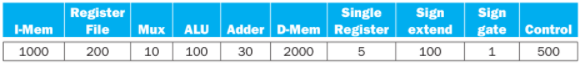
\includegraphics[scale=0.6]{q10_image}\\\end{center}
Suppose doubling the number of general purpose registers from 32 to 64 would reduce the number of lw and sw instruction by 12\%, but increase the latency of the register file from 150 ps to 160 ps and double the cost from 200 to 400. (Use the instruction mix from Exercise 4.8 and ignore the other effects on the ISA discussed in Exercise 2.18.)

\begin{enumerate}[(a)]
    \item What is the speedup achieved by adding this improvement?\\
    \textbf{Work:}
    \begin{center}
        Clocktime Before Impr. = 250 + 150 + 25 + 200 + 150 + 5 + 30 + 20 + 50 + 50 = 930 ps\\
        Clocktime After Impr. = 250 + 160 + 25 + 200 + 150 + 5 + 30 + 20 + 50 + 50 = 940 ps\\
        Speedup achieved = (930 / 100) / (940/97) = 0.95\\
        \fbox{\begin{minipage}{15em}
            \begin{center}
                \Large{\textbf{Answer: 0.95}}
            \end{center}
        \end{minipage}}
    \end{center}

    \item Compare the change in performance to the change in cost.\\
    \textbf{Work:}
    \begin{center}
        Cost w/o Impr. = 1000 + 10 + 200 + 100 + 2000 + 30 + 5 + 1 + 100 + 500 = 3946\\
        Cost / Clocktime = 3946 / 930 = 4.24\\
        Cost w/ Impr. = 1000 + 10 + 400 + 100 + 2000 + 30 + 5 + 1 + 100 + 500 = 4146\\
        Cost / Clocktime = 4146 / 940 = 4.38\\
        Change in cost: 4.38 - 4.24 = 0.14\\[0.15in]
        Performace = 1 / Latency\\
        Performance w/o Impr. = $1 / (930 * 100 * 10^{-12}) = 10.75 * 10^6$\\
        Performance w/ Impr. = $1 / (940 * 96 * 10^{-12}) = 11.08 * 10^6$\\
        Change in performance: 11.08 - 10.75 = 0.33\\[0.15in]
        The cost ratio is = 4.38 / 4.24 = 1.03\\
        The performance ratio is = 11.08 / 10.75 = 1.03\\[0.15in]
        \fbox{\begin{minipage}{15em}
            \begin{center}
                \Large{\textbf{Answer: Both are 1.03}}
            \end{center}
        \end{minipage}}
    \end{center}
    
    \item Given the cost/performance ratios you just calculated, describe a situation where it makes sense to add more registers and describe a situation where it doesn't make sense to add more registers.\\
    Increasing the number of registers has led to decreased costs and improved performance. However, prioritizing performance may require accepting higher costs. 
    Utilizing more registers to decrease the number of instructions can enhance performance but at a higher cost. 
    Contrarily, if reducing costs is the priority, using fewer registers might be necessary, even though this can lead to a greater number of instructions
     and subsequently impact latency, ultimately lowering performance. In conclusion, more registers for better performance and fewer registers for cost efficiency.
\end{enumerate}

\setcounter{subsubsection}{15}
\subsubsection{Question 16}
In this exercise, we examine how pipelining affects the clock cycle time of the processor. Problems in this exercise assume that individual stages of the datapath have the following latencies:
\begin{center}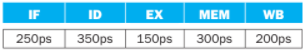
\includegraphics[scale=0.68]{q16_image1}\\\end{center}
Also, assume that instructions executed by the processor are broken down as follows:
\begin{center}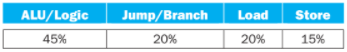
\includegraphics[scale=0.6]{q16_image2}\\\end{center}

\begin{enumerate}[(a)]
    \item What is the clock cycle time in a pipelined and non-pipelined processor?\\
    \textbf{Answer:}
    \begin{center}
        For a pipelined processor, the clock cycle time is the time it takes to complete the longest stage.\\ 
        \fbox{\begin{minipage}{20em}
            \begin{center}
                \Large{\textbf{Answer: Pipelined is 350ps}}
            \end{center}
        \end{minipage}}\\[0.15in]       
        For a non-pipelined processor, the clock cycle time is the sum of all the stages.\\
        Total time = IF + ID + EX + MEM + WB = 250 + 150 + 200 + 500 + 150 = 1250ps\\
        \fbox{\begin{minipage}{25em}
            \begin{center}
                \Large{\textbf{Answer: Non-Pipelined is 1250ps}}
            \end{center}
        \end{minipage}}
    \end{center}

    \item What is the total latency of an lw instruction in a pipelined and non-pipelined processor?
    \textbf{Answer:}
    \begin{center}
        Piplined Processor:
        The total latency = \# Cycles * \#Clock Cycles\\
        The total latency = 5 * 350ps = 1750ps\\
        \fbox{\begin{minipage}{20em}
            \begin{center}
                \Large{\textbf{Answer: Pipelined is 1750ps}}
            \end{center}
        \end{minipage}}\\[0.15in]

        Non-Pipelined Processor:
        The total latency = IF + ID + EX + MEM + WB\\
        The total latency = 250ps + 350ps + 150ps + 300ps + 200ps = 1250ps\\
        \fbox{\begin{minipage}{25em}
            \begin{center}
                \Large{\textbf{Answer: Non-Pipelined is 1250ps}}
            \end{center}
        \end{minipage}}
    \end{center}

    \item If we can split one stage of the pipelined datapath into two new stages, each with half the latency of the original stage, which stage would you split and what is the new clock cycle time of the processor?\\
    \textbf{Answer:}
    \begin{center}
    The stage I would split is the longest stage, which is the ID stage. 
    The new clock cycle time would be 300ps, which is the max of the new one, which is the MEM\\
    \fbox{\begin{minipage}{20em}
        \begin{center}
            \Large{\textbf{Answer: 300ps}}
        \end{center}
    \end{minipage}}
    \end{center}
    

    \item Assuming there are no stalls or hazards, what is the utilization of the data memory?\\
    \textbf{Answer:}
    \begin{center}
        The utilization is load + store\\
        Total utilization  = 20\% + 15\% = 35\%\\
        \fbox{\begin{minipage}{20em}
            \begin{center}
                \Large{\textbf{Answer: 35\%}}
            \end{center}
        \end{minipage}}
    \end{center}

    \item Assuming there are no stalls or hazards, what is the utilization of the write-register port of the "Registers" unit?\\
    \textbf{Answer:}
    \begin{center}
        The utilization is the LW utilization + ALU utilization.\\
        20\% + 45\% = 65\%\\
        \fbox{\begin{minipage}{20em}
            \begin{center}
                \Large{\textbf{Answer: 65\%}}
            \end{center}
        \end{minipage}}
    \end{center}
\end{enumerate}
\end{document}